\chapter{Tecnologie di interesse}\label{cap:tecnologie}

\intro{In questa sezione viene presentata una panoramica di base delle tecnologie oggetto del mio tirocinio, al fine
di descrivere in modo chiaro e conciso i concetti di base e le caratteristiche principali delle tecnologie utilizzate
nel progetto di stage e oggetto di studio autonomo e autodidatta.}

\section{Blockchain: concetti base}\label{sec:tecnologie-blockchain}

\subsection{Introduzione}\label{sec:tecnologie-blockchain-introduzione}

La \glsfirstoccur{\gls{blockchaing}} è una tecnologia che permette di memorizzare dati in maniera decentralizzata e distribuita.
Essa è una struttura dati che si comporta come un registro distribuito, salvando le informazioni in modo sicuro ed immutabile.
La struttura è stata introdotta nel 2008 da Satoshi Nakamoto, che ha pubblicato il suo white paper \textit{Bitcoin: A Peer-to-Peer Electronic Cash System}.
Nel 2009 è stato pubblicato il primo \textit{software} \glsfirstoccur{\gls{opensourceg}} per la \textit{blockchain}, Bitcoin, che ha permesso di creare una moneta digitale decentralizzata. \\

A tal fine, non si devono confondere le cosiddette criptovalute con la \textit{blockchain}. Di fatto, quest'ultima è solo la struttura che permette lo scambio di beni di qualsiasi tipo,
in modo sicuro, registrato ed immutabile. Una criptovaluta è invece una moneta digitale, che può essere scambiata con altre monete digitali o con beni fisici.
Essendo lo standard \textit{blockchain} \textit{open source}, è possibile crearne di nuove con molta facilità.

Normalmente, viene utilizzata per memorizzare transazioni finanziarie, ma può essere utilizzata per memorizzare qualsiasi tipo di informazione.
Un altro suo nome è \textit{distributed ledger technology} (DLT), che indica che le sue informazioni sono registrate come su un libro mastro, in cui le singole componenti della rete,
definite nodi, possono accedere e modificare i dati, stabilendo se questi sono validi o meno. 

\subsection{Blocco}\label{sec:tecnologie-blockchain-blocco}

I dati delle \textit{blockchain} sono strutturati in singoli blocchi, ciascuno contenente uno specifico set di informazioni.
Ogni blocco è collegato al precedente tramite un hash, che ne garantisce l'immutabilità.
I blocchi sono collegati in una catena, che viene aggiornata ogni volta che viene aggiunto un nuovo blocco.
Nello specifico, possiamo dettagliare una struttura formata dai seguenti (come descritto in figura~\ref{fig:blocco}):
\begin{itemize}
    \item blocchi di dati;
    \item nonce, un numero generato casualmente alla creazione del blocco;
    \item l'hash del blocco precedente;
    \item il numero della transazione;
    \item \textit{timestamp} di generazione del blocco (data e ora).
\end{itemize} 

\begin{figure}[ht]
    \centering
    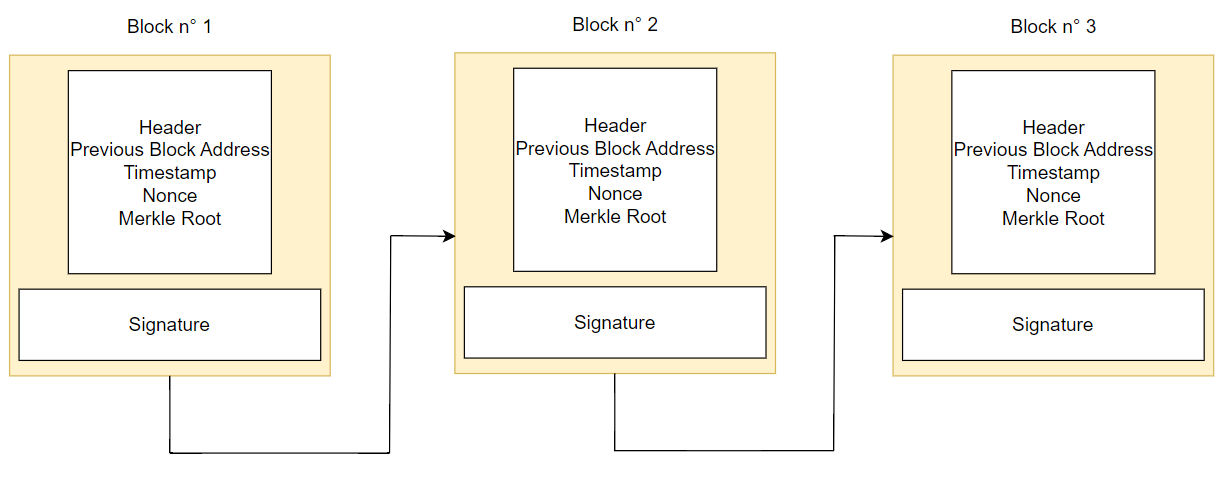
\includegraphics[width=0.6\textwidth, alt={Blocco all'interno di una blockchain}]{immagini/blocco.png}
    \caption{Blockchain vista come blocchi a catena}\label{fig:blocco}
\end{figure}

Per verificare l'integrità dei dati memorizzati, vengono usate delle strutture dati chiamati \textit{Merkle trees}, in cui ogni foglia rappresenta l'hash della transazione.
Le foglie vengono poi raggruppate in coppie, e l'hash di ogni coppia viene calcolato e memorizzato in un nodo superiore.
Il processo si ripete, fino a raggiungere la radice dell'albero, che rappresenta l'hash di tutte le transazioni contenute nel blocco.

\subsection{Transazione}\label{sec:tecnologie-blockchain-transazione}

Una transazione all'interno di una \textit{blockchain} comporta il trasferimento di beni digitali, che possono essere valute, token, o qualsiasi altro tipo di informazione.
In questo senso, possiamo individuare vari componenti del processo di transazione:
\begin{itemize}
    \item{gli utenti}, che avviano le transazioni firmandole digitalmente con la propria chiave privata;
    \item{i \textit{miners}}, che attraverso un processo specifico definito come \textit{mining}, verificano la validità delle transazioni e le includono nel blocco successivo. 
    \item{i nodi}, che convalidano i blocchi di transazioni inviati dai miners prima che vengano aggiunti alle \textit{blockchain}.
\end{itemize}

Nello specifico, possiamo descrivere una transazione in questo modo:
\begin{enumerate}
    \item l'utente avvia la transazione creando una firma digitale utilizzando la propria chiave privata. La firma dimostra che l'utente ha il diritto di inviare i beni;
    \item la transazione viene trasmessa alla rete di nodi o computer che eseguono il \textit{software} della \textit{blockchain}. Ogni nodo riceve la transazione e la aggiunge a un pool di transazioni non confermate;
    \item i nodi della rete convalidano la transazione per assicurarsi che il mittente abbia fondi sufficienti per completare la transazione e che questa sia conforme alle regole del protocollo \textit{blockchain};
    \item una volta che un numero sufficiente di nodi ha convalidato la transazione, questa viene aggiunta a un nuovo blocco di transazioni, insieme ad altre transazioni convalidate di recente;
    \item il blocco di transazioni viene aggiunto alla \textit{blockchain} in un processo chiamato \textit{mining}. L'estrazione comporta la risoluzione di complesse equazioni matematiche per creare un nuovo blocco, il che richiede una grande potenza di calcolo;
    \item una volta aggiunto il nuovo blocco alla \textit{blockchain}, la transazione viene considerata confermata e i beni vengono trasferiti dall'indirizzo del mittente a quello del destinatario. La transazione è ora registrata in modo permanente sul libro mastro della \textit{blockchain}, che può essere visualizzato e verificato da chiunque abbia accesso alla rete;
\end{enumerate}

\subsection{Wallet}\label{sec:tecnologie-blockchain-wallet}

Un \textit{wallet}, detto anche \textit{portafoglio}, è un software che permette di memorizzare e gestire le chiavi private e pubbliche, e di inviare e ricevere transazioni.
In particolare, possiamo più propriamente definirli portachiavi, in quanto non contengono realmente i beni digitali, ma le chiavi utilizzate per accedervi.
L'utente dispone in ogni momento di:
\begin{itemize}
    \item una chiave pubblica, usata per inviare messaggi e ricevere pagamenti. È un codice univoco che identifica l'utente;
    \item una chiave privata, usata per firmare i messaggi e per accedere ai propri beni digitali. È un codice segreto che deve essere conservato in modo sicuro.
\end{itemize} 

Ogni \textit{wallet} dispone di una frase segreta, che contiene tutte le informazioni necessarie per recuperare ed accedere ai fondi del proprio portachiavi.

Inoltre, dispone di un proprio indirizzo, matematicamente derivato dalla stessa chiave pubblica mediante l'operazione di \textit{hashing}, con una lunghezza di 160 bit.
Ciascuno è \textit{pseudonimo}, in quanto non appartiene nello specifico ad una persona, ma non è completamente anonimo. \\
È importante tenere la chiave privata in un luogo sicuro e non condividerla con nessuno, in quanto è l'unica cosa che garantisce l'accesso ai propri fondi.
Distinguiamo due tipi di \textit{wallet}:
\begin{itemize}
    \item \textit{hot wallet}, che sono i portafogli online, dunque più vulnerabili al rischio di \textit{hacking};
    \item \textit{cold wallet}, che sono i portafogli offline, quindi considerati più sicuri, in quanto si collegano ad Internet principalmente per effettuare le transazioni.
\end{itemize}

\subsection{Mining}\label{sec:tecnologie-blockchain-mining}

Il processo di \textit{mining} consente di creare nuovi blocchi sulla catena, al fine di convalidare le transazioni e ottenere nuove criptovalute come ricompensa per il proprio `sforzo'.
Questo obiettivo viene raggiunto attraverso un processo chiamato `consenso-, che prevede la risoluzione di complessi puzzle matematici utilizzando la potenza di calcolo.
Il miner che riesce a risolvere il puzzle prima degli altri, vince il diritto di aggiungere il blocco alla \textit{blockchain}. \\

Questo processo è composto da due fasi:
\begin{itemize}
    \item \textit{hashing}, che consiste nella risoluzione di un \textit{puzzle} matematico, che consiste nel trovare un numero che, una volta applicata una funzione di hash, abbia un valore inferiore ad un valore prefissato. Il valore di questo numero viene chiamato \textit{nonce};
    \item \textit{ricerca del consenso}, che consiste nella verifica della validità del blocco, che viene effettuata da tutti i nodi della rete. Se il blocco è valido, viene aggiunto alla \textit{blockchain}.
\end{itemize}

I minatori (miners) utilizzano un software speciale per risolvere il problema matematico incredibilmente complesso 
di trovare un \textit{nonce} che generi un hash accettato. Poiché il \textit{nonce} è di soli 32 bit e l'hash di 256, ci sono circa quattro miliardi 
di possibili combinazioni nonce-hash che devono essere estratte prima di trovare quella giusta. \\

Quando un blocco viene estratto con successo, la modifica viene accettata da tutti i nodi della rete e il \textit{miner} viene ricompensato finanziariamente. 
Il primo minatore che risolve il puzzle e aggiunge un nuovo blocco alla \textit{blockchain} viene ricompensato con un blocco di criptovaluta di nuovo conio.
Il processo richiede un software specializzato e una grande potenza di calcolo, che può essere ottenuta utilizzando un computer o un gruppo di computer con grosso dispendio di energia e risorse.

\subsection{Algoritmi di consenso}\label{sec:tecnologie-blockchain-algoritmi}
Il meccanismo di ricerca di consenso prevede numerose varianti, che differiscono per il modo in cui i nodi della rete si accordano per aggiungere un nuovo blocco alla \textit{blockchain}.\\
Possiamo principalmente distinguere:
\begin{enumerate}
    \item\textit{{Proof of Work (PoW)}}, basato nella ricerca di un hash (una stringa di numeri e lettere) che soddisfa una determinata condizione, detta target. Tale condizione richiede 
    che l'hash del nuovo blocco sia inferiore a un determinato valore. Questo valore viene stabilito in base alla difficoltà della \textit{blockchain}, che viene regolata automaticamente per mantenere 
    il tempo medio di creazione di un nuovo blocco costante. Questo processo è descritto visivamente dalla figura~\ref{fig:pow}.

    Il primo miner che trova correttamente l'hash del blocco viene ricompensato in criptovaluta per il lavoro svolto.
    Questo meccanismo garantisce sicurezza nella rete, perché rende difficile ad un attaccante malintenzionato
    compromettere la sicurezza della rete non avendo la stessa potenza di calcolo.
    
    Questa è attualmente utilizzata in \textit{Bitcoin}, in cui il tempo medio della formazione di blocchi è di 10 minuti circa, oppure la piattaforma \textit{Ethereum}, altro importante esempio di blockchain.
    Si consideri che ne esistono varie tipologie, in cui ciascuna cerca di ridurre il consumo energetico dando prova del lavoro svolto (\textit{Meaningful}) oppure assicurandosi che
    i nodi abbiano calcolato correttamente dopo un certo tempo (\textit{Delayed}).
    Il principale svantaggio del PoW è che richiede un elevato consumo energetico, che può essere risolto con l'utilizzo di algoritmi di consenso alternativi.

    \begin{figure}[ht]
        \centering
        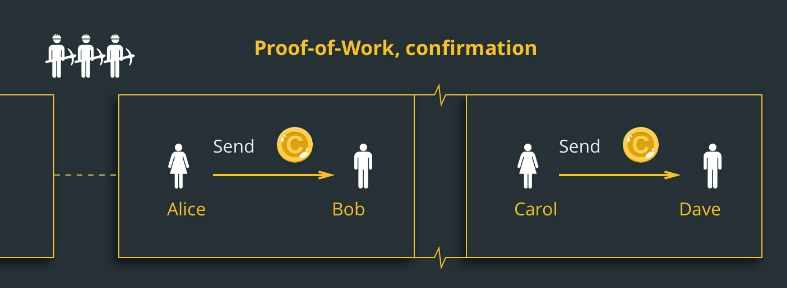
\includegraphics[width=0.6\textwidth, alt={Come avviene il processo di conferma in Proof of Work}]{immagini/proof-of-work.png}
        \caption{Processo di conferma in Proof of Work}\label{fig:pow}
    \end{figure}

    \item\textit{{Proof of Stake (PoS)}}, che si si basa sulla detenzione di una certa quantità di criptovaluta come garanzia per la validazione delle transazioni. 
    L'alto consumo di energia dell'algoritmo precedente ha portato ad algoritmi come il \textit{Proof of Stake}, i nodi della rete bloccano una certa quantità di criptovaluta come `punteggio'
    per dimostrare che hanno un interesse nella corretta validazione delle transazioni. 
    Questo punteggio viene utilizzato come base per la selezione del nodo che convalida la transazione successiva. 
    
    A differenza del \textit{PoW}, non ci sono \textit{miner} coinvolti nel processo. Al loro posto, i partecipanti alla rete che 
    vogliono essere coinvolti nella verifica della validità delle transazioni e nella creazione di blocchi nella rete 
    devono detenere una certa quota nella rete, per esempio mettendo una certa quantità di moneta della rete in un portafoglio collegato 
    alla sua \textit{blockchain}. Questo processo è noto come `placing a stake' o `staking', che può essere tradotto come il fatto di mettere i propri interessi in gioco. 
    
    Pertanto, le reti PoS sono basate su algoritmi deterministici, il che significa che i validatori dei blocchi sono eletti a seconda della natura della posta in gioco. 
    Pur risultando meno intensiva in termini di energia rispetto alla \textit{PoW}, il sistema risulta essere sbilanciato a favore dei produttori di blocchi oppure a favore degli utenti ricchi, 
    poiché i validatori con più moneta hanno più possibilità di essere eletti. 
    Alcune varianti di questo algoritmo prevedono infatti di scegliere dei nodi delegati per convalidare le transazioni e avere più controllo (\textit{Delegated}), 
    oppure di scegliere i validatori in base alla quantità di moneta che hanno investito (\textit{Proof of Burn}).

\end{enumerate}

\clearpage

\subsection{Tipi}\label{sec:tecnologie-blockchain-tipi}
Una prima categorizzazione delle \textit{blockchain} avviene distinguendole in base ai permessi. Nello specifico:
\begin{itemize}
    \item \textit{permissioned}, in cui i nodi della rete sono controllati da un ente centrale, che può essere un'azienda, un'organizzazione o un'istituzione.
    Esse limitano l'accesso alla rete a determinati nodi e possono anche limitare i diritti di tali nodi su tale rete. Le identità degli utenti di una blockchain autorizzata sono note agli altri utenti della blockchain autorizzata.
    Queste sono spesso utilizzate da aziende per la gestione di dati sensibili o convalida di transazioni;
    \item \textit{permissionless}, che non richiedono alcun permesso per partecipare e permettono agli utenti di essere pseudoanonimi 
    (usando uno pseudonimo non si rivela alcun dettaglio relativo all'identità personale) e non restringono i permessi dei nodi. Queste ultime tendono ad essere più sicure delle precedenti, avendo vari nodi che convalidano le singole transazioni.
    Di fatto, sono usate dalle varie \textit{blockchain}, come ad esempio quella di Bitcoin.
\end{itemize}

Fatta tale premessa, possiamo distinguere:
\begin{itemize}
    \item \textit{public}, in cui chiunque abbia accesso alla rete può partecipare e diventare un nodo autorizzato nella \textit{blockchain}. Di fatto sono sicure, ma non anonime e molto meno scalabili.
    Una loro futura implementazione sarà all'interno dei sistemi di votazioni elettroniche.
    \item \textit{private}, in cui i singoli nodi sono controllati da un ente centrale, che opera in una rete chiusa e, come tali, restringono la natura di blockchain, dato che richiede controllo centralizzato dei singoli nodi per poter funzionare.
    Queste sono utilizzate da parte di alcune banche per la gestione dei loro sistemi di pagamento.
    \item \textit{hybrid}, in cui alcuni nodi sono pubblici e altri sono privati, normalmente utilizzata per eseguire convalide delle transazioni presenti al suo interno.
    Microsoft utilizza una blockchain di identità digitale basata sul meccanismo ibrido.
    \item \textit{consortium}, all'interno della quale i nodi sono controllati da un ente centrale, ma la rete è aperta a tutti i membri del consorzio, portando anche qui ad una privatizzazione e centralizzazione della rete.
    IBM sta utilizzando una piattaforma basata sulla gestione dei pagamenti per banche ed aziende partner.
\end{itemize}

\section{Blockchain: concetti avanzati}\label{sec:tecnologie-blockchain-avanzate}

\subsection{Token}\label{sec:tecnologie-blockchain-avanzate-token}
Possiamo definire i \textit{token} come unità di valore accettate da una comunità e costruite su una \textit{blockchain} pre-esistente (dunque, non possono essere minati).
Possono essere usati per rappresentare asset fisici come l'oro o l'immobiliare, oppure per rappresentare beni digitali 
come i dati o i diritti di accesso a servizi. Essendo registrati su una \textit{blockchain}, sono immutabili e possono essere trasferiti in modo sicuro e trasparente da un proprietario all'altro. \\

Per utilizzare i token, gli utenti devono prima avere un portafoglio digitale, ovvero un'interfaccia che consente loro 
di accedere alla \textit{blockchain} e interagire con essa. Una volta che un utente ha un portafoglio, 
può ricevere e inviare token. Per ricevere i token, l'utente deve fornire il proprio indirizzo del portafoglio al mittente, 
che poi invia i \textit{token} all'indirizzo fornito. Per inviare i token, l'utente deve avere abbastanza \textit{token} nel proprio portafoglio e deve conoscere l'indirizzo del destinatario a cui inviare i token. \\

Ogni bene viene considerato \textit{asset}, in quanto non riproducibile e non falsificabile, esistente solo in forma digitale e quindi non fisica. 
Un \textit{token} può essere lanciato sul mercato tramite un \textit{initial coin offering} (ICO),
che è un'offerta pubblica iniziale di \textit{token}, al fine di finanziare nuovi progetti e comprenderne il nuovo valore.
\\ 
Come per le \textit{blockchain}, gli asset non sono regolamentati da un organo centrale, pertanto è possibile raccogliere fondi senza nuovi intermediari e così creare
nuovi progetti, adeguatamente documentati tramite un \textit{white paper} che descrive il progetto e il suo funzionamento. 
Il loro processo di creazione dei \textit{token} nelle \textit{blockchain} viene definito come \textit{minting}, in cui un creatore mette a disposizione un certo numero di token,
che possono essere acquistati dai partecipanti. \\

Principalmente, i \textit{token} possono essere classificati in base al loro scopo:
\begin{itemize}
    \item \textit{Utility token}, che consentono di acquistare un determinato bene o servizio e conferisce al titolare un diritto di opzione per l'acquisto o somministrazione di cose o per la fornitura di servizi (attuali o futuri). 
    \item \textit{Security token}, che sono \textit{token} che rappresentano un diritto di proprietà su un bene fisico o digitale.
    \item \textit{Payment token}, più comunemente noti come `crypto'. Come si può intuire, questi \textit{token} sono utilizzati per acquistare e vendere beni e pagare le commissioni delle transazioni basate sulla blockchain senza la necessità di un intermediario.
\end{itemize}

I token, principalmente, sono caratterizzati dal fatto di essere spendibili e scambiabili con altri beni dal valore equivalente, ossia `fungibili'.
In questo senso, è possibile citare:
\begin{itemize}
    \item \textit{token fungibili (fungible tokens)}, che hanno la caratteristica di essere non uniche, divisibili e avere un chiaro valore di mercato, quindi scambiabili sempre con altri beni dello stesso valore;
    \item \textit{token non fungibili (non fungible token/NFT)}, beni fisici o digitali unici e irripetibili. Questi vengono definiti come tali in quanto non possono essere scambiati con altri beni dello stesso valore,
    e per natura delle stesse \textit{blockchain}, sono considerati immutabili. Infatti, l'utente, disponendo di un \textit{wallet}, può creare in qualsiasi momento un bene considerabile come unico, pagando una commissione al momento dell'acquisto del bene.
    Questo particolare tipo di \textit{token} è molto utilizzato per la vendita di beni come opere d'arte, musica, videogiochi, per loro natura non contraffabile dato lo scambio tramite blockchain.
\end{itemize}

La loro creazione è vincolata da alcuni standard, stabilità della comunità della \textit{blockchain} \textit{Ethereum}, che ne vincola la creazione tramite \textit{smart contract},
che sono dei contratti che vengono eseguiti sulla \textit{blockchain} e che possono essere scritti in vari linguaggi di programmazione. \\
Di seguito i principali standard di riferimento che stabiliscono precisamente i parametri della loro creazione:
\begin{itemize}
    \item \textit{ERC-20}, che è il più diffuso e utilizzato standard per i token, che consente di creare \textit{token} che possono essere trasferiti tra gli utenti. 
    Questo stabilisce che un contratto esponga un saldo, un'opzione di trasferimento, un'opzione di approvazione e un evento di trasferimento;
    \item \textit{ERC-721}, che è uno standard per i \textit{token} non divisibili (NFT), che rappresentano un bene unico non scambiabile in altri modi.
    Di base utilizza gli stessi parametri del precedente, ma possiede un campo specifico che indica chi è il proprietario;
    \item \textit{ERC-1155}, che è uno standard per i \textit{token} divisibili e non divisibili e riunisce a livello di dati un supporto comune con funzione di trasferimento e di approvazione anche in blocco.
\end{itemize} 

\subsection{Tokenizzazione}\label{sec:tecnologie-blockchain-avanziate-tokenizzazione}
La tokenizzazione è il processo di rappresentazione di un bene o di un'attività in forma digitale attraverso l'emissione di un \textit{token} su una \textit{blockchain}. 
In altre parole, si tratta di convertire un bene fisico o immateriale in un asset digitale che può essere negoziato e scambiato in modo decentralizzato.
La combinazione con la \textit{blockchain} potrebbe aprire nuove prospettive per l'ottimizzazione dei processi aziendali, che includono più partner, e l'introduzione di nuovi modelli di \textit{business}. 
Poiché la tokenizzazione è un processo decentralizzato, non è necessario un intermediario per la creazione e la gestione di un \textit{token} e questo facilita la creazione di nuovi beni,
sapendo che la verifica viene effettuata da tutti i partecipanti della rete ed ogni bene è considerato unico. \\

Esistono diversi tipi di asset da considerare, i quali saranno poi successivamente convertiti in token:
\begin{itemize}
    \item{\textit{Asset finanziari}}, che rappresentano un diritto di proprietà su un bene fisico o digitale. Il concetto della finanza decentralizzata sta emergendo come \textit{DeFi (Decentralized Finance)},
    in cui i beni vengono spostati su \textit{blockchain} a seconda della loro natura. Infatti, come per i \textit{token} i beni acquistano una fungibilità e possono essere scambiati tra utenti;
    \item{\textit{Asset immobiliari}}, che rappresentano un bene fisico, come un immobile, che può essere tokenizzato e quindi diventare un bene digitale. 
    Questi beni sono fungibili e come tali hanno un valore tendenzialmente fisso, che può essere soggetto a variazioni nel tempo;
    \item{\textit{beni intangibili (intangibles)}}, come diritti di proprietà intellettuale o i citati beni collezionabili,
    e quindi acquisire grazie alla natura di \textit{blockchain} un valore unico e verificato.
\end{itemize} 

Si può quindi comprendere che la tokenizzazione può potenzialmente trasformare tutto in un bene con un valore, permettendo di avere dei prezzi equi stabiliti dalle vere esigenze del mercato,
riducendo i costi di gestione essendo un sistema scalabile e sicuro che lo gestisce, permettendo l'aumento della liquidità, avendo sempre degli investitori pronti a scambiare i token, in modo trasparente
e senza intermediari, riducendo notevolmente i tempi di scambio rispetto ai beni tradizionali.

\subsection{Smart contract}\label{sec:tecnologiechain-avanziate-smart-contract}
Gli \textit{smart contract} (o contratti intelligenti) sono programmi che automatizzano le azioni richieste in un accordo o contratto, considerate tracciate e irreversibili. 
Essi sono programmi informatici auto-eseguibili che vengono eseguiti su una \textit{blockchain}, che automatizzano ed eseguono le clausole contrattuali in modo sicuro, trasparente e immutabile, senza la necessità di intermediari.
Il loro funzionamento è regolato dal libro mastro centrale di \textit{blockchain}, in cui i partecipanti devono firmare crittograficamente la loro partecipazione, fornendo precisamente i loro indirizzi di riferimento 
e codificando lo scambio delle informazioni secondo gli standard definiti nella sezione precedente. \\

Gli \textit{smart contract} sono stati sviluppati per risolvere i problemi di affidabilità e sicurezza dei contratti tradizionali, che sono soggetti a errori umani, mancanza di trasparenza e vulnerabilità.
Il loro funzionamento segue generalmente questo schema:
\begin{enumerate}
    \item un utente avvia una transazione dal proprio portafoglio \textit{blockchain};
    \item la transazione arriva al database distribuito, dove viene confermata l'identità del portafoglio dell'utente;
    \item la transazione, che può essere un trasferimento di fondi e comprende il codice che definisce il tipo di transazione da eseguire, viene approvata;
    \item questa viene eseguita come blocco all'interno della \textit{blockchain}.
\end{enumerate}
Nella figura~\ref{fig:smart-contract} è possibile vedere un esempio di funzionamento. \\

Principalmente, questi vengono utilizzati nella piattaforma \glsfirstoccur{\gls{ethereumg}}, dove i contratti vengono scritti in linguaggio di programmazione \textit{Solidity}, 
che è un linguaggio di programmazione orientato agli oggetti basato su \textit{C++},
eseguiti sulla piattaforma \textit{Ethereum Virtual Machine (EVM)}, che ne consente l'esecuzione in modo scalabile regolata dagli standard precedenti.
Ogniqualvolta venga eseguita una transazione, si ha un costo pagato in \textit{gas}, costo in termini di energia necessaria per eseguire la transazione, che viene calcolato in base al numero di operazioni eseguite
e pone un limite al numero di transazioni che possono essere eseguite in un dato periodo di tempo. \\

\begin{figure}[ht]
    \centering
    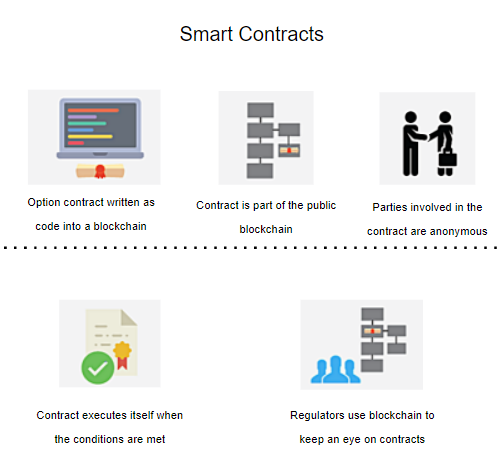
\includegraphics[width=0.6\textwidth, alt={Come funziona uno Smart Contract}]{immagini/smart-contract.png}
    \caption{Funzionamento di uno Smart Contract}\label{fig:smart-contract}
\end{figure}

\newpage

Possiamo citare alcuni esempi di applicazione di \textit{smart contract}:
\begin{itemize}
    \item \textit{smart legal contracts}, legalmente applicabili e richiedono alle parti di soddisfare i loro obblighi contrattuali.
    Per creare alcuni contratti legali intelligenti, le parti coinvolte lavorano sul codice del contratto intelligente (o lo fanno i loro sviluppatori di software) finché non si accordano sui termini e sulle condizioni dell'accordo;
    \item \textit{decentralized autonomous organizations (DAO)}, che sono organizzazioni che funzionano in modo decentralizzato e autonomo, senza un leader centrale e \textit{open-source}, ma regolate da un contratto intelligente.
    All'interno delle \textit{blockchain} vengono organizzate delle votazioni, che possono essere eseguite da tutti i partecipanti, che possono votare per o contro una proposta,
    oppure garantire il corretto scambio dei beni digitali all'interno della piattaforma, prevenendo possibili vulnerabilità;
    \item \textit{crowdfunding}, che è un metodo di finanziamento di progetti e aziende, in cui le persone possono contribuire con denaro o beni, in cambio di un premio o di un prodotto finale;
    \item \textit{logical applicative contracts}, che sono contratti che possono essere utilizzati per eseguire operazioni logiche, come la verifica di un dato e l'esecuzione di un'altra operazione,
    oppure gestire un sistema di pagamento o beni di scambio, garantendo la tracciabilità e la trasparenza di ogni bene alla consegna.
\end{itemize}

I contratti rimangono aggiornati grazie all'uso di \textit{oracoli}, sistemi che permettono di ottenere informazioni esterne alla \textit{blockchain}, come il valore di un bene o il valore di un'azione,
attraverso l'uso di \glsfirstoccur{\gls{apig}} o di altri sistemi di comunicazione. In questo modo, il contratto mantiene la sua funzionalità interagendo in maniera ibrida con il mondo esterno; questi vengono definiti come \textit{hybrid smart contracts}, 
combinando un'infrastruttura \textit{on-chain} con un'infrastruttura \textit{off-chain}.
Il loro utilizzo, per quanto utile, deve essere attentamente bilanciato, sia in termini di veridicità dei dati che di sicurezza, in quanto possono essere soggetti a compromissione o di scalabilità, per cui è necessario
un'attenta valutazione dei rischi.

\clearpage

\subsection{Vulnerabilità e sicurezza}\label{sec:tecnologie-blockchain-avanzate-vulnerabilita-sicurezza}

Le \textit{blockchain} sono soggette a vulnerabilità, che possono essere sfruttate per ottenere informazioni o per compromettere il sistema.
Il linguaggio \textit{Solidity}, infatti, è un linguaggio che richiede particolare attenzione nella scrittura del codice, in quanto è possibile sfruttare alcune vulnerabilità date dal mancato controllo delle operazioni fatte, ciascuna
delle quali comporta una transazione e scambio di criptovaluta, pubblicamente visibile e come tale tracciabile ed attaccabile in ogni momento. 
Ogni dato deve essere opportunamente criptato e protetto, in quanto è possibile ottenere informazioni sensibili come \textit{password} oppure \textit{chiavi private} di un portafoglio, che permettono di accedere ai fondi
e di eseguire transazioni. \\
Di seguito verrà esaminato un insieme di problemi comuni che si possono verificare all'interno di un contratto intelligente, dovuti principalmente al mancato controllo e convalida 
dei dati in ingresso e in uscita, portando allo sfruttamento di vulnerabilità nell'ordine in cui vengono eseguite le operazioni.

\begin{itemize}
    \item \textbf{re-entrancy}: è un problema importante che può verificarsi ogni volta si chiami una funzione di un contratto esterno; se il contratto esterno è malevolo, può essere sfruttato per eseguire
    delle chiamate ricorsive. Ogni volta che il contratto esterno `rientrerà' nella funzione, riceverà la stessa quantità di fondi. Al termine dell'esecuzione, l'importo inviato sarà probabilmente più volte superiore a quello previsto.
    Questo problema può essere risolto utilizzando la funzione \textit{transfer} o \textit{send} per inviare fondi, in quanto queste funzioni eseguono un'operazione \textit{throw} in caso di errore, interrompendo l'esecuzione del contratto
    e lanciando immediatamente un'eccezione che interrompe l'esecuzione del contratto. Un altro modo è di controllare l'ordine delle chiamate delle funzioni, 
    introducendo l'uso dei cosiddetti \textit{modifier}, che permettono di controllare l'ordine di esecuzione delle funzioni oppure attraverso l'uso delle istruzioni \textit{assert} e \textit{require}, che fermano l'esecuzione del codice 
    qualora determinate condizioni non vengano rispettate (ad esempio, se il valore di un dato è negativo oppure per controllare gli indirizzi che eseguono le stesse transazioni);
    \item \textbf{integer overflow/underflow}: è un problema che si verifica quando si tenta di eseguire un'operazione aritmetica che produce un risultato troppo grande o troppo piccolo per essere rappresentato.
    Questo problema può essere sfruttato per ottenere un risultato diverso da quello atteso, ad esempio, se si tenta di sottrarre un numero più grande da uno più piccolo, il risultato sarà un numero molto grande, che potrebbe essere
    utilizzato per realizzare una transazione malevola ed ottenere un guadagno. Il problema può essere risolto sfruttando le ultime versioni del linguaggio \textit{Solidity};
    \item \textbf{Denial of Service (DoS)}: è un attacco che mira a rendere un servizio non disponibile per gli utenti legittimi, attraverso l'invio di un numero elevato di richieste, che possono essere eseguite in maniera
    automatica. Il problema si verifica qualora esistano delle chiamate a contratti esterni non controllati oppure se si utilizzano cicli \textit{for} o \textit{while} con un numero di iterazioni elevato. 
    Questo problema può essere risolto attraverso l'uso di \textit{gas limit} e \textit{gas price}, che permettono di limitare il numero di operazioni eseguibili e di fissare un prezzo limite per ogni operazione;
    \item \textbf{timestamp dependency}: è un problema che si verifica quando si utilizza il \textit{timestamp} per eseguire operazioni, ad esempio, per controllare se un contratto è scaduto oppure per controllare se un utente ha eseguito
    un'operazione in un determinato intervallo di tempo. Questo problema può essere sfruttato per eseguire un'operazione in un momento diverso da quello previsto, ad esempio, se si utilizza il timestamp per controllare se un contratto
    è scaduto, un utente potrebbe eseguire un'operazione prima del tempo previsto. Questo problema può essere risolto utilizzando il \textit{block number}, che permette di controllare il numero di blocchi eseguiti, oppure utilizzando
    il \textit{block hash}, che permette di controllare l'hash del blocco corrente e verificare se è stato modificato;
    \item \textbf{transaction-ordering dependency (front running)}: è un problema che si verifica quando un utente esegue un'operazione prima di un altro utente, ad esempio, se un utente esegue un'operazione di acquisto di un bene
    ad un prezzo più basso rispetto ad un altro utente, l'utente che esegue l'operazione per primo otterrà il bene ad un prezzo più basso. Questo problema può essere risolto utilizzando il \textit{block number} oppure il \textit{block hash}
    come visto in precedenza;
\end{itemize}

Altri accorgimenti che si possono adottare sono il controllo della visibilità fornita alle funzioni, che possono essere \textit{public}, \textit{private}, \textit{internal} o \textit{external},
intendendo rispettivamente che la funzione può essere chiamata da chiunque, solo all'interno del contratto, solo all'interno del contratto e dai contratti che ereditano il contratto oppure solo dai contratti che ereditano il contratto.
Anche i valori di ritorno delle funzioni, se non controllati, possono scatenare dei problemi importanti di sicurezza, ad esempio, se una funzione restituisce un valore booleano, è possibile che un utente malevolo possa
sfruttare questo valore per eseguire un'operazione non prevista, iniettando del codice indesiderato oppure eseguendo transazioni nulle, volte a consumare risorse della rete ed ottenere un guadagno esterno.
I contratti sono, per loro natura, deterministici e le operazioni devono essere eseguite precisamente nello stesso ordine da tutti i nodi della rete, in modo da ottenere lo stesso risultato.
Risulta quindi fondamentale considerare e controllare ciascuna di queste importanti problematiche, evitando che si generino situazioni in cui un nodo della rete può prendere il controllo di numerose operazioni,
idealmente prendendo il controllo della maggioranza della rete (problema noto come \textit{51\% attack}) oppure prendendo il controllo di numerosi nodi creando molteplici identità fasulle (problema noto come \textit{Sybil attack}).

\subsection{Scalabilità}\label{sec:tecnologie-blockchain-avanzate-scalabilita}
Le blockchain sono preziose per il fatto di essere un sistema deterministico e con un grado di affidabilità molto elevato, generalmente neutro e verificabile da parte dell'utente finale.
In questo contesto, è fondamentale parlare del cosiddetto \textit{blockchain trilemma}, che è un problema di scelta tra tre caratteristiche fondamentali di una blockchain: decentralizzazione, sicurezza e scalabilità.
Infatti, decentralizzare significa mantenere un vasto numero di nodi sulla rete, senza però alcun controllo da parte di un ente centrale, 
mantenendo allo stesso modo un alto numero di transazioni in modo scalabile e una robustezza ai possibili partecipanti della rete. \\

In questo senso, si cerca di trovare un compromesso tra le tre caratteristiche, che è possibile ottenere l'aggiunta di ridondanza dei dati anche al di fuori della blockchain principale,
cercando di bilanciare quanto possibile il consenso sui nodi distribuiti non intaccando il livello di libertà offerto ma anche aumentare il livello di dati trasmessi.
Per questo, il nucleo scalabilità permette di introdurre numerose soluzioni al fine di migliorare le prestazioni della \textit{blockchain}, dividendo però la \textit{blockchain} in vari strati, definiti come \textit{layer}.
\begin{itemize}
    \item{\textit{Layer 0}}, che è la \textit{blockchain} principale, che contiene i dati e le transazioni;
    \item{\textit{Layer 1}}, che è il livello responsabile della sicurezza e della scalabilità, che contiene i nodi che eseguono le transazioni e che sono responsabili della validazione;
    \item{\textit{Layer 2}}, noto anche come livello di esecuzione, in cui si hanno i contratti intelligenti e le applicazioni che vengono eseguite sulla \textit{blockchain};
    \item{\textit{Layer 3}}, noto anche come livello applicativo, che contiene le applicazioni decentralizzate (\glsfirstoccur{\gls{dappg}}), eseguite sulle \textit{blockchain} e che interagiscono con gli utenti.
\end{itemize}

Comunemente, le soluzioni di scalabilità cercano di intervenire in vari modi:
\begin{itemize}
    \item{\textit{Sharding}}, che è una tecnica di scalabilità che consente di dividere la \textit{blockchain} in più parti, chiamate \textit{shards}, che possono essere gestite da nodi diversi e aumentando
    la dimensione dei singoli blocchi e la loro frequenza di creazione. Questa si effettua comunemente per il \textit{Layer 1}.
    \item{\textit{Sidechains}}, che sono \textit{blockchain} secondarie che vengono utilizzate per eseguire transazioni parallele, che vengono poi sincronizzate con la \textit{blockchain} principale.
    In questo ambito, soluzioni comuni includono i \textit{canali di stato (state channels)}, che sono dei contratti intelligenti che permettono di eseguire transazioni tra due parti, senza che queste siano visibili sulla blockchain principale,
    e i \textit{canali di pagamento (payment channels)}, che migliorano la comunicazione bidirezionale delle transazioni eseguendole sulla \textit{blockchain} secondaria e dandone traccia sulla principale.
\end{itemize}

\section{Self Sovereign Identity}\label{sec:self-sovereign-identity}

La \glsfirstoccur{\gls{ssig}} è un approccio all'identità digitale che dà agli individui 
il controllo sulle informazioni che usano per dimostrare chi sono a siti web, servizi e applicazioni in tutto il web. 
Senza l'\textit{SSI}, gli individui con \textit{account} (identità) persistenti su Internet devono affidarsi a una serie di fornitori terzi, come Facebook, Google e altri,
che hanno il controllo delle informazioni associate alla loro identità. \\

Esistono molti modi per implementare l'\textit{SSI}  utilizzando le chiavi crittografiche e ne analizzeremo due.
\begin{itemize}
    \item l'utilizzo di firme digitali, attraverso un processo di \textit{firma digitale}, che permette di firmare un documento con una chiave privata, e di verificare la firma con la chiave pubblica;
    \item \glsfirstoccur{\gls{didg}}, che è un identificatore univoco alfanumerico per un soggetto, che può essere utilizzato per identificare una persona, un'organizzazione, un dispositivo, un servizio, un documento, ecc.
\end{itemize}  

Le parti coinvolte in questo processo sono principalmente tre:
\begin{enumerate}
    \item {\textit{emittente}, detto anche \textit{holder}}, ossia l'entità che emette una credenziale, ad esempio un documento d'identità governativo;
    \item {\textit{titolare}, detto anche \textit{issuer}}, ossia il proprietario della credenziale, cioè l'entità su cui l'emittente genera la credenziale;
    \item {\textit{verificatore}, detto anche \textit{verifier}}, cioè l'entità che controlla la validità e l'autenticità della credenziale presentata dal titolare.
\end{enumerate}  

Il processo di riconoscimento è descritto dalla figura~\ref{fig:ssi}.

\begin{figure}[ht]
    \centering
    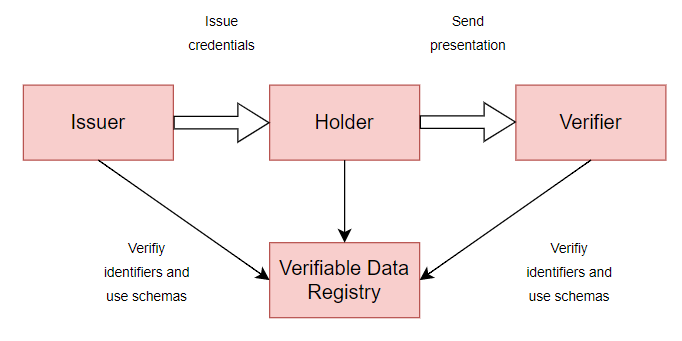
\includegraphics[width=0.6\textwidth, alt={Come funziona il riconoscimento nella SSI}]{immagini/ssi.png}
    \caption{Processo di riconoscimento di una credenziale SSI}\label{fig:ssi}.
\end{figure}

Lo scopo principale di questa tecnologia è consentire agli utenti un'esistenza indipendente da provider terzi, 
permettendo loro di controllare la propria identità in modo sicuro e accedendovi senza dover affidarsi a terzi. \\
Inoltre, i sistemi e gli algoritmi che la supportano devono essere trasparenti, mantenendo le informazioni in modo trasparente e permanente, rendendo però semplice 
la portabilità e l'interoperabilità di queste all'interno delle varie piattaforme. \\

La tecnologia blockchain, per mezzo della sua natura decentralizzata, permette di creare un sistema di identità digitale che soddisfi questi requisiti.
In particolare:
\begin{itemize}
    \item il titolare della credenziale possiede il suo \textit{Decentralized Identifier} firmato dalla propria coppia di chiavi che certifica la sua identità;
    \item l'emittente fornisce delle \glsfirstoccur{\gls{vcg}}, che certificano in modo digitale e crittograficamente protetto la validità del proprio ruolo;
    \item il verificatore controlla che, tramite ciascun blocco, sia stata rilasciata una \textit{VC} valida e che il titolare sia il legittimo possessore di quella VC.\@
\end{itemize}  

L'obiettivo principale è quello di fornire un utilizzo delle tecnologie \textit{blockchain} tali da permettere agli utenti 
di selezionare quali credenziali mostrare (\textit{selective disclosure o divulgazione selettiva}),
secondo opportuni standard definiti gradualmente dall'organizzazione internazionale \glsfirstoccur{\gls{w3cg}}, tra cui il citato \textit{VC}.\@

\subsection{Tipi e applicazioni}\label{sec:self-sovereign-identity-tipi-applicazioni}

Il concetto di \textit{SSI} è stato introdotto nel 2015 da \textit{Sovrin Foundation}, che ha sviluppato il protocollo \textit{Sovrin},
organizzazione privata senza scopo di lucro che ha creato la prima rete di identità auto-sovrana, diventato poi standard \textit{W3C}. 
Esso si basa sul protocollo è \textit{Hyperledger Indy}, che è un \glsfirstoccur{\gls{frameworkg}} \textit{open source} per la creazione di \textit{SSI} basato su \textit{blockchain}
che fornisce strumenti, librerie e componenti riutilizzabili per fornire identità digitali legate al mondo \textit{blockchain}, 
come ad esempio la firma digitale e la crittografia. \\

Questo è il principale, ma possiamo definire un insieme di standard 
utilizzati al fine di garantire agli utenti di possedere e controllare in modo indipendente la propria identità digitale, gestendo come vengono
condivise le proprie informazioni. La particolarità di questi protocolli è di comunicare gli uni con gli altri attraverso messaggi crittografati:
\begin{itemize}
    \item \textit{DID (Decentralized Identifier)}, che consente di creare identificativi digitali decentralizzati come citato supportano
    e permettono di identificare i soggetti in modo resistente alla falsificazione, autenticando le informazioni in modo sicuro;
    \item \textit{VC (Verifiable Credentials)}, che consente di gestire attestazioni verificati, quindi insiemi di informazioni che un individuo
    possiede o controlla, dimostrando che l'attestazione è stata rilasciata da un emittente autorizzato. Questo all'interno delle \textit{blockchain}
    garantisce che ciascun nodo e parte in gioco sia chi dice di essere senza ledere la decentralizzazione alla base;
    \item \glsfirstoccur{\gls{zkpg}}, che consente di dimostrare la conoscenza di una proprietà di un dato, senza rivelare alcun dettaglio relativo.
    Questa tecnologia è considerata a sé stante un'innovazione tecnologica, che permette attraverso l'individuazione di parti precise,
    la certezza che solo chi conosce l'informazione può correttamente rispondere alle domande poste senza rivelare i propri dati.
\end{itemize}

Attualmente, la tecnologia \textit{SSI} prevede una graduale implementazione in sistemi di autenticazione e
in generale di accesso ai servizi pubblici, permettendo all'utente un ulteriore controllo
sui dati trasmessi rivelandoli solo a parti autorizzate.
Questo risulta particolarmente utile nel settore sanitario, legislativo (garantendo certezza di identità e di voto) e finanziario,
permettendo di ridurre i costi di gestione e di mantenimento dei dati, oltre che di ridurre i tempi di accesso ai servizi.
Il principale organo promotore è la \textit{Decentralized Identity Foundation (DIF)}, che ha come obiettivo quello di creare
un ecosistema di identità digitali decentralizzate, promuovendo integrazioni, progetti e nuove idee in questo ambito. 

\section{Zero Knowledge Proof}\label{sec:zero-knowledge-proof}
Definita anche come prova a conoscenza zero, è una tecnologia che permette di dimostrare la conoscenza di una proprietà di un dato,
senza rivelare alcun dettaglio relativo.
Occorre definire le parti coinvolte:
\begin{itemize}
    \item \textit{Prover}, ossia l'entità che prova la conoscenza di alcune informazioni riservate. 
    L'informazione segreta è il `testimone' (\textit{witness}) della prova e la presunta conoscenza del testimone da parte del prover stabilisce un insieme di domande a cui può rispondere solo chi conosce l'informazione. 
    \item \textit{Verifier}, ossia l'entità che verifica la correttezza della prova. Lui si occupa di scegliere a caso la sfida (\textit{challenge}) e di verificare la risposta del prover.
    La risposta del prover permette al verificatore di controllare se il primo ha davvero accesso al testimone. La verifica segue visivamente dalla figura~\ref{fig:zkp}. 
    Per assicurarsi che il prover non stia indovinando alla cieca e non ottenga le risposte corrette per caso, il verificatore sceglie altre domande da porre.
\end{itemize}

\begin{figure}[ht] 
    \centering
    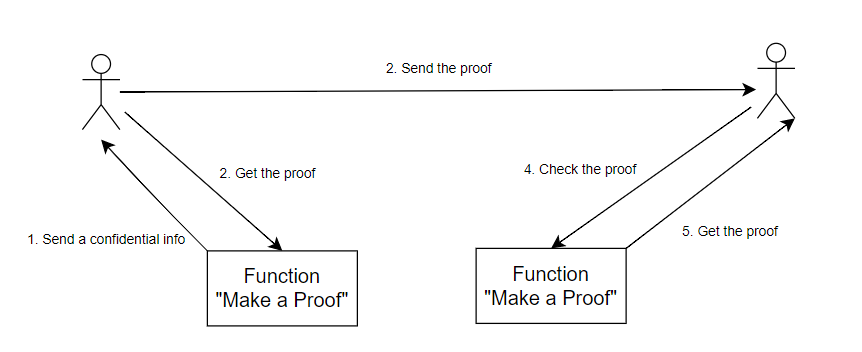
\includegraphics[width=0.6\textwidth, alt={Come funziona la verifica nella ZKP}]{immagini/zkp.png}
    \caption{Processo di verifica di una ZKP}\label{fig:zkp}
\end{figure}

A livello di transazioni, la \textit{ZKP} è utilizzata per garantire la sicurezza con certezza che le transazioni siano valide (\textit{validity proofs}), tramite la presenza del testimone tipicamente basato su calcoli polinomiali o
prossimità ad un insieme di valori, come ad esempio la distanza di Hamming. Le transazioni possono essere invalidate in ogni momento tramite le \textit{fraud proofs}, che dimostrano che la transazione è stata effettuata in modo illegittimo.
Queste ultime confrontano i \textit{Merkle trees} delle transazioni e verificano che l'\textit{hash} corrisponda a quella originale. \\

Di fatto, ogni prova deve dimostrare di essere completa, pertanto è necessario che il verificatore sia in grado di verificare che la risposta del \textit{prover} sia corretta,
dimostrando questa affermazione con solidità, in modo da non lasciare spazio a dubbi e a falsi positivi, senza trasmettere alcun dato (a conoscenza zero).
L'idea principale della \textit{ZKP} è presupporre di non fidarsi di nessuno (\textit{zero trust}), al fine di garantire la sicurezza delle informazioni. 
In questo modo, ciascun utente viene monitorato a livello di privilegi, accessi e dati, senza che nessuno possa accedere senza dimostrare di averne il permesso. \\

\subsection{Tipi e applicazioni}\label{sec:zero-knowledge-proof-tipi-applicazioni}
Esistono diverse implementazioni di \textit{ZKP}, ognuna delle quali presenta un proprio compromesso in termini di dimensione della prova, tempo del \textit{prover}, tempo di verifica e altro ancora. 
I principali tipi sono: 
\begin{itemize}
    \item{\textit{zk-SNARK}}, acronimo di \textit{Zero Knowledge Succinct Non-interactive Argument of Knowledge}, prova di dimensioni ridotte e facile da verificare. Essa è stata sviluppata dalle piattaforme \textit{Zcash} e \textit{Ethereum} 
    utilizzando le curve ellittiche, che presuppongono che sia impossibile trovare il logaritmo discreto di un elemento casuale della curva ellittica a partire da un punto base pubblicamente noto. Il calcolo delle curve ellittiche è meno dispendioso dal punto di vista computazionale rispetto al calcolo delle funzioni di hashing.
    \item{\textit{zk-STARK}}, acronimo di \textit{Zero Knowledge Succinct Transparent Argument of Knowledge}, tipo di prova crittografica che richiede un'interazione minima o nulla tra il \textit{prover} e il verificatore. I vantaggi principali delle STARK rispetto alle SNARK sono che hanno tempi di prover rapidi e sono più facili da scalare in quanto offrono una maggiore potenza di calcolo.
    Essa è stata sviluppata dalla piattaforma \textit{Horizen} utilizzando le \textit{curve ellittiche}, che presuppongono che sia impossibile trovare il logaritmo discreto di un elemento casuale della curva di \textit{Weierstrass} a partire da un punto base pubblicamente noto. Il calcolo delle curve di \textit{Weierstrass} è più dispendioso dal punto di vista computazionale rispetto al calcolo delle curve ellittiche.
\end{itemize}

All'interno delle blockchain, vengono utilizzati all'interno delle \textit{sidechain} secondo il sistema delle \textit{zk-Rollup}, che permettono di eseguire transazioni su una \textit{blockchain} laterale (\textit{sidechain}) senza doverle scrivere su questa.
In altre parole, con uno \textit{zk-rollup}, le transazioni vengono `confezionate' in un'unica transazione che viene elaborata sulla \textit{blockchain}, riducendo il carico di lavoro richiesto alla rete. 
Inoltre, grazie all'utilizzo delle \textit{Zero Knowledge Proof}, le transazioni vengono verificate in modo sicuro, senza rivelare alcuna informazione sulle transazioni stesse.
 
Principalmente, queste vengono utilizzate in sistemi di scalabilità \textit{layer-2}, al fine di memorizzare solo il minimo numero previsto di transazioni (\textit{rollup}),
oppure memorizzando solamente un hash sulla catena per proteggere i dati del libro mastro (validium), oppure scegliere come salvarli per ogni transazione (\textit{volition}).
Alcuni casi d'uso possibili di applicazione di questa tecnologia possono essere:
\begin{itemize}
    \item{pagamenti anonimi}
    \item{protezione dell'identità}
    \item{autenticazione}
    \item{archiviazione di dati sensibili}
\end{itemize}

L'utilizzo combinato con la \textit{Self Sovereign Identity} è particolarmente interessante perché consente di garantire la \textit{privacy} e la sicurezza delle informazioni personali degli utenti.
In particolare, è possibile garantire di conoscere le parti in gioco nella rete poiché verificate
in modo sicuro e privato tramite credenziali certificate, scegliendo anzi quali informazioni rivelare e senza
dover rivelare alcuno dei propri dati per dimostrare di possederli. 